\newpage
\section{Blokschema niveau}
\label{Block_schema}
Met de subsystemen kan nu een blokschema ontworpen worden. Dit blokschema is weergegeven in Figuur \ref{fig:Blok_schema_1_top_level}. Dit blokschema bestaat uit zeven subsystemen die elke verder uitgewerkt kunnen worden. Doordat meerdere blokken van het blokschema uitgezet of in een laag verbruik stand geplaatst kunnen worden zullen deze blokken minder vermogen verbruiken.

\begin{figure}[H]
    \centering
    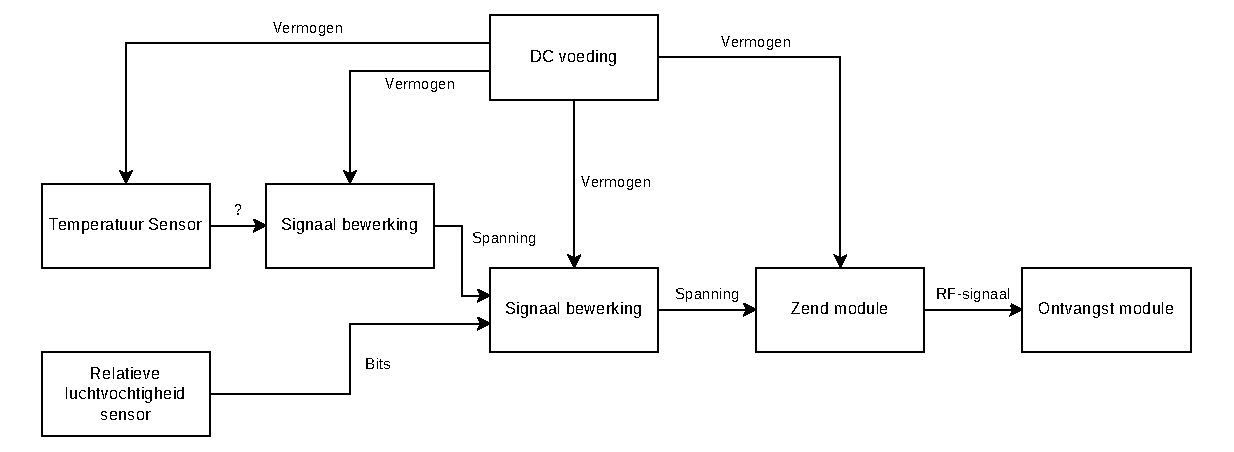
\includegraphics[width=0.85\linewidth]{pictures/Blok_schema_systeem_ontwerp_1.drawio.pdf}
    \caption{Blokschema opgebouwd uit alle subsystemen.}
    \label{fig:Blok_schema_1_top_level}
\end{figure}

\subsection{Temperatuursensor}
Zoals is beschreven in hoofdstuk \ref{Systeem_niveau}: Systeem niveau, is het niet mogelijk om de sensor uit te schakelen. Hierdoor is het nodig dat er goed nagedacht wordt over hoe de temperatuur sensor zo energiezuinig mogelijk ontworpen wordt. Het type sensor en de aansturing daarvan spelen een grote rol hierin. Dit wordt allemaal beschreven in hoofdstuk \ref{Circuit_niveau}: Circuit niveau. Hierdoor is het nog niet mogelijk om een berekening te doen van het vermogensverbruik. Daarom is er voor nu besloten dat de temperatuursensor maximaal 1 mW mag verbruiken. Dit is gedaan om de rest van de applicatie zo veel mogelijk van het vermogensbudget te geven. Voor de nauwkeurigheid van de sensor zijn er minimaal 600 meet stappen nodig. Dit betekent dus dat de ruis minimaal kleiner moet zijn dan 1/600ste van het maximale bereik van de sensor. Anders kan de sensor de specificaties niet behalen. Om van Piek ruis naar effectieve ruis te gaan wordt er gedeeld met een factor 6. Hierom is er besloten dat de ruis maximaal 1/3600ste van de sensors maximale bereik. Met deze eis is er een minimale SNR van 71,1 dB nodig. 

In de specificaties is vast gesteld dat er minimaal elke tien seconden één meting plaats moet vinden. Dit zorgt voor een bandbreedte van minimale 0,1 Hz. Omdat


Omdat uit de specificaties is bepaald dat er minimaal één meting elke 10 seconden gedaan moet worden 

\subsection{Signaalbewerking}
De uitgang van de temperatuursensor kan niet direct uitgelezen worden door het digitale signaalbewerkingsblok. Hiervoor moet eerst het signaal versterkt worden door een Signaal bewerkingsblok. De versterking hangt af van de signalen die het digitale Signaal bewerkingsblok kan verwerken. Om de applicatie energiezuinig te houden mag dit Signaal bewerkingsblok 1 mW gebruiken om ervoor te zorgen dat de zend module zoveel mogelijk heeft om informatie goed te verzenden. Om dit te bereiken is misschien nodig om dit blok uit en aan te kunnen schakelen. Hierom moet er rekening mee gehouden in de verdere ontwerpstappen.
\\
\newline
Het signaalbewerkingsblok dat is aangesloten op de relatieve luchtvochtigheidssensor en het hierboven vermelde signaalbewerkingsblok. Heeft twee ingangen waarvan één digitaal is en de andere een analoog signaal is. Hierdoor moet dit blok in het digitale domein te werk gaan. Omdat dit in het digitale domein plaatsvindt, is het mogelijk om eenvoudig de absolute luchtvochtigheid te berekenen. Nadat deze berekening is gebeurd wordt deze informatie omgevormd naar een analoog signaal om de zendmodule hiermee aan te sturen. Door twee omvormingen die in het signaalbewerkingsblok plaats vinden is er bepaald dat er 2 mW aan energie verbruik nodig is om dit te doen.

\subsection{Relatieve luchtvochtigheid sensor} 
Zoals is beschreven in hoofdstuk \ref{Systeem_niveau}: Systeem niveau, is dit een blok met een digitale uitgang. Dit zorgt ervoor dat er in applicatie een digitale chip moet zijn om de informatie van de Relatieve luchtvochtigheid Sensor uit te lezen en te kunnen verwerken. Het verbruik en nauwkeurigheid zijn de belangrijkste eigenschappen voor de sensor keuze.

\subsection{Zendmodule}
Het zendmodule blok verwerkt de signalen die hij binnen krijgt naar een RF-signaal. Dit RF-signaal wordt via een antenne verstuurd naar de Ontvangst module. De frequentie waarop de zendmodule zijn informatie verstuurd zal gebeuren op een openbare band \cite{RF_banden}. Dit zorgt ervoor dat er geen zendlicentie nodig is om de applicatie te gebruiken. Het energieverbruik van de applicatie mag niet boven de 10 mW uit komen. Om dit te voorkomen wordt gedoeld op een energie verbruik van 5 mW voor het zend module blok.

\subsection{Energieverdeling}
Het vermogen is nu als volgt, verdeeld over de blokken van het blokschema. Dit is zichtbaar in Tabel \ref{tab:Energie_verbruik_blok_schema}.
\begin{table}[H]
    \centering
    \begin{tabular}{|c|c|}
        \hline
        \textbf{Blokken} & \textbf{Energie verbruik} \\ \hline
        Temperatuur sensor & 1 mW \\ \hline
        Signaal bewerking  & 1 mW \\ \hline
        Digitale signaal bewerking & 2 mW \\ \hline
        Relatieve luchtvochtigheid sensor & 100 $\mu$W \\ \hline
        Zend module & 5 mW \\ \hline
        totaal  & 9,1 mW \\ \hline

    \end{tabular}
    \caption{Vermogens verdeling van de applicatie op blokschema niveau.}
    \label{tab:Energie_verbruik_blok_schema}
\end{table}

\newpage
\subsection{flowchart}  % voor jochem
Om de programmastructuur voor de digitale verwerking inzichtelijk te maken en om het systeem zo efficiënt mogelijk te ontwerpen is een flow chart gemaakt, te zien in Figuur \ref{fig:flow_chart}.
\newline
\begin{figure}[H]
    \centering
    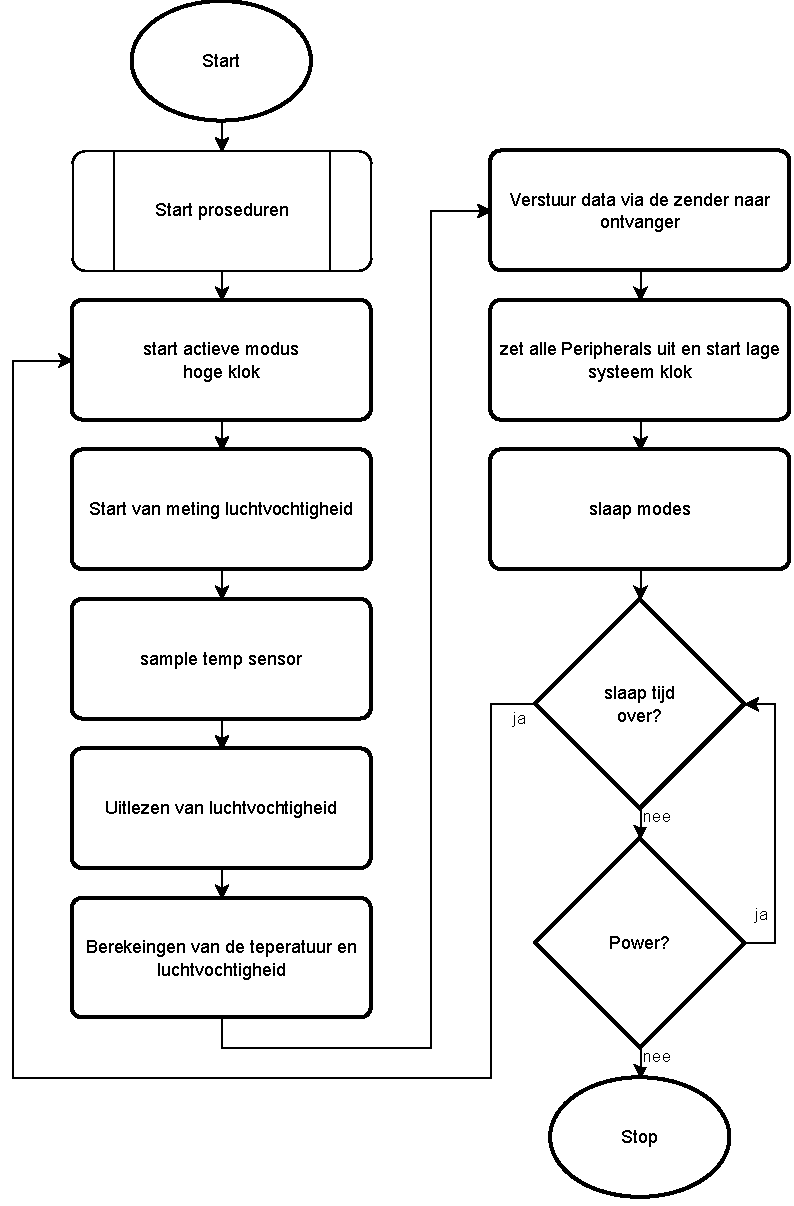
\includegraphics[width=0.65\linewidth]{pictures/jochem_flowchart.drawio.pdf}
    \caption{Flow chart digitale signaal bewerking.}
    \label{fig:flow_chart}
\end{figure}

Tijdens de start procedure zullen de digitale systemen correct ingesteld worden voor het doen van de metingen, en zullen eventueel overbodige systemen uitgeschakeld worden om energie te besparen. Omdat er slechts elke 10 seconde een meting gedaan hoeft te worden zal het systeem het grootste deel van de tijd in slaap modus kunnen zijn. Dat wil zeggen alle systemen uit staan en alleen een systeem om weer in actieve modus te komen nog aan zal blijven staan. Tijdens de actieve modes zal de systeemklok hoog zijn, het verbruik van het digitale systeem heeft namelijk een lineair verband met de kloksnelheid. Om de andere subsystemen zoals de zender zo kort mogelijk aan te hebben, en het verbruik van deze systemen zo laag mogelijk te houden moet de actieve modes zo kort mogelijk zijn. Door een hoge kloksnelheid te kiezen neemt het totale gebruikte vermogen van het digitale systeem niet of nauwelijks toe, maar kan de verwerking van de sensor gegevens wel sneller gedaan worden en hoeven deze systemen minder lang aan te staan waardoor deze systemen zuiniger zijn. Het is wel van belang om de tijd in active modes zo efficiënt mogelijk te gebruiken, dat wil zeggen zo min mogelijk wachten, want wachten betekent klokslagen die niet nodig zijn en verspilde energie. Het beperken van wachten wordt bijvoorbeeld gedaan door de luchtvochtigheidssensor een meting te laten starten en daarna alvast de temperatuur sensor uit te lezen, zodat hierna de resultaten van de luchtvochtigheidssensor klaarstaan en hier niet op gewacht hoeft te worden. Zodra de gegevens verzamelt zijn zal de zender aangezet worden en worden de gegevens verstuurd, vervolgens zullen alle systemen weer uitgeschakeld of in slaap modus gezet worden om te wachten tot de volgende meting gedaan moet worden.


\subsection{Vereenvoudigen van blokschema}
Het blokschema wat ontworpen is uit de subsystemen is nog niet ver genoeg opgedeeld. Dit zorgt ervoor dat er een nieuw blokschema ontworpen moet worden wat gebaseerd is op het eerste schema, maar dan uit meer basisfuncties bestaat om het ontwerpen van het circuit in hoofdstuk \ref{Circuit_niveau}: Circuitniveau makkelijker en duidelijker te maken. Dit blokschema is weergegeven in Figuur \ref{fig:bigger_blok_schematic}. Het blok ADC is de analoog naar digitaal conversie waarin gezorgd wordt dat het analoog signaal verder bewerkt kan worden door de digitale bewerking. Daarnaast is er het blok DAC waarin de conversie van digitaal naar analoog in plaats vindt, zodat de zender het signaal kan begrijpen.

\begin{figure}[H]
    \centering
    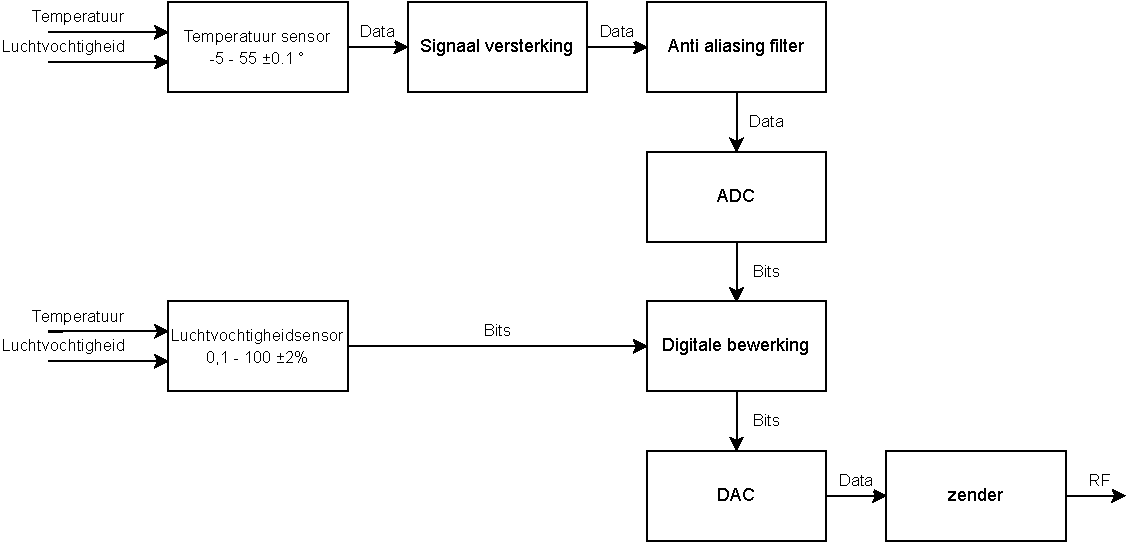
\includegraphics[width=1\linewidth]{pictures/blokschema.drawio.pdf}
    \caption{Blokschema opgebouwd uit meer basis functies.}
    \label{fig:bigger_blok_schematic}
\end{figure}